\documentclass[12pt,a4paper,twoside,spanish]{book}

\usepackage{Formato}

\title{Tesis 2 Introducción }
\author{Aaron Sújar}



\begin{document}
\frontmatter


\pagenumbering{roman}

%\include{ack}
\thispagestyle{empty}
\chapter*{Acronyms}

\begin{acronym}
\acro{B-rep}{representación superficial}
\acro{Bangor}{Bangor University}
\acro{DQS}{dual quaternion skinning}
\acro{CAD}{diseño asistido por computador}
\acro{COR}{centros de rotación}
\acro{Courseware}{aplicación de entrenamiento}
\acro{DICOM}{Imagen y Comunicación Digital en Medicina}
\acro{DOF}{grados de libertad}
\acro{E/S}{Entrada/Salida}
\acro{EASA}{Agencia Europea de Seguridad Aérea}
\acro{FEM}{método de elementos finitos}
\acro{FORTH}{Foundation for Research and Technology - Hellas}
\acro{CGAL}{Computational Geometry Algorithms Library}
\acro{GLSL}{OpenGL Shading Language}
\acro{GMRV}{Grupo de Modelado y Realidad Virtual}
\acro{GPL}{GNU General Public License}
\acro{GPU}{unidad de procesamiento gráfico}
\acro{ITGVPH}{Integrated Toolkit for Generation of VPH Models}
\acro{INRIA}{Institut National de Recherche en Informatique et en Automatique}
\acro{IRM}{imagen por resonancia magnética}
\acro{IU}{interfaz de usuario}
\acro{joints}{articulaciones virtuales}
\acro{kvp}{tensión de pico}
\acro{kV}{kV}{kilovoltio}
\acro{keV}{keV}{kiloelectronvoltio}
\acro{LGPL}{GNU Lesser General Public License}
\acro{LBS}{linear blending skinning}
\acro{mAs}{mAs}{miliamperio por segundo}
\acro{MoCap}{captura de movimientos}
\acro{RA}{anestesia regional}
\acro{RAAs}{Regional Anaesthesia Assistant}
\acro{RAM}{Random Access Memory}
\acro{RASim}{Regional Anaesthesia Simulator}
\acro{RASimAs}{Regional Anaesthesia Simulator and Assistant}
\acro{RDT}{triangulación restringida de delaunay}
\acro{RV}{realidad virtual}
\acro{RWTH}{RWTH Aachen University}
\acro{SBS}{Spherical Blend Skinning}
\acro{SINTEF}{Stiftelsen for industriell og teknisk forskning}
\acro{SG}{Sensegraphics}
\acro{SOFA}{Simulation Open Framework Architecture}
\acro{TASMIP}{TASMIP}{tungsten anode spectral model using interpolating polynomials}
\acro{TC}{tomografía axial computarizada}
\acro{TPTVPH}{Toolkit for Pose Transforms of VPH Models}
\acro{tracker}{dispositivo de seguimiento}
\acro{tabla hash}{Spatial Hash Table}
\acro{UKA-IMI}{Department of Medical Informatics: Uniklinik RWTH Aachen}
\acro{URJC}{Universidad Rey Juan Carlos}
\acro{US}{ultrasonidos} 
\acro{ViSTA}{Virtual Reality Toolkit}
\acro{VPH}{pacientes virtuales}
\acro{VTU}{formato de Visualization Toolkit}
\acro{WP}{paquetes de trabajos}
\acro{X3D}{formato Extensible 3D}
\acro{XML}{Extensible Markup Language}
\acro{ZPD}{zona de desarrollo próximo}













\end{acronym}


\tableofcontents
\listoffigures
 
\listoftables
\mainmatter
\chapter{Introducción} 

\label{cap:intro}


% \todo{Entiendo que quieres comentar la importancia de los gráficos por computador en el mundo actual. Primero te comento errores cometidos y luego te propongo soluciones:
% 1. La generación de imágenes hace referencia solo al proceso de renderizado. El área de conocimiento son los gráficos por computar, estos incluyen animación, modelado, post-proceso.
% 2. El mundo del la generaicón y tratamiento de imagenes es demasiado amplio. Tú deberías centrarlo en el campo del los gráficos 3D (aquellos en los que la imagen generada nos permite de alguna manera (claves perpetúales captar la profundidad))
% 3. Todo el mundo sabe que los gráficos 3D estan tanformando el mundo del ocio (peliculas de animación, videojuegos) y el mundo profesional (por cierto no hablaria del mundo profesional, hablaria de la cientcia, el foramción, analisis de datos, interacción hombre máquina ...). Pero en este párrafo no concretas estas aportaciones. Ocio: ciene y videojuegos, Apredizaje: gamificación, entremiento en entornos seguros. Ciencia: Visualización y análisis de datos.... 
% Solución:
% No hables de los graficos por computador. Tu tesis se enmarca en la RV. La RV utiliza los graficos por computador y muchas otras displinas. 
% Te estoy metiendo comentarios largos por si te pueden ayudar con futuras redacciones. }

Durante los últimos años, el término de \ac{RV} se ha incorporado a nuestro lenguaje cotidiano. Esto es debido a la gran penetración que están teniendo este tipo de sistemas en nuestra vida privada y, cada vez más, en distintos ámbitos profesionales. Podemos encontrar ejemplos de estas aplicaciones en sectores tan diversos como: el mundo del ocio, donde los videojuegos son el máximo exponente del uso de estas tecnologías; el campo del entrenamiento profesional, en el que la \ac{RV} permite el desarrollo de destrezas no cognitivas en entornos controlados\cite{PATEL2017266.e7}; el ámbito científico, donde estos sistemas facilitan la compresión de datos complejos mediante el uso de entornos inmersos \cite{usher2018}. Dado el gran número de campos de aplicación y de tecnologías utilizadas, no resulta fácil indicar de forma unívoca qué caracteriza una aplicación de \ac{RV}. En la bibliografía, pueden encontrarse distintas definiciones del término:

\begin{center}
    \begin{minipage}{0.9\linewidth}
        %\vspace{5pt}%margen superior de minipage
        {\small
\emph{Virtual reality is a high-end user-computer interface that
involves real-time simulation and interactions through
multiple sensorial channels.}
        }
        \begin{flushright}
            (Burdea and Coiffet, 2003: \cite{burdea2003virtual})
        \end{flushright}
        %\vspace{5pt}%margen inferior de la minipage
    \end{minipage}
    
    \begin{minipage}{0.9\linewidth}
        %\vspace{5pt}%margen superior de minipage
        {\small
\emph{VR is the science and technology required for a user
to feel present, via perceptive, cognitive and functional
immersion and interaction, in a (computer) generated
environment. }
        }
        \begin{flushright}
            (Casarin et al., 2015: \cite{kuntz2015middlevr})
        \end{flushright}
        %\vspace{5pt}%margen inferior de la minipage
    \end{minipage}
    
\end{center}
%
%\todo{1.La realidad virtual no es una subcampo del los graficos por computdor.2.En algún lugar hay que hablar de la multidisciplinaridad de este campo (ingeniería, ciencias de la computación, psicología, graficos por computador...). Puede ir despues de la definición.}
% Este comentario esta para que no sea un parrafo nuevo
Tal y como se desprende de las definiciones anteriores, las aplicaciones \ac{RV} se caracterizan por presentar al usuario un entorno virtual a través de varios canales sensoriales, permitiéndole interactuar con el mismo y generando en él, una sensación de inmersión y presencia \cite{Jerald:2015}. Estos objetivos imprimen a este campo una naturaleza altamente multidisciplinar. La \ac{RV} se asienta en disciplinas como la ingeniería mecánica, los gráficos por computador, la percepción, la computación de altas prestaciones... De esta forma, el desarrollo de estas aplicaciones requiere naturalmente de expertos en distintas áreas de conocimiento.  

%\todo{ojo con afirmar cosas que no estan justificadas como "inmersión completa" o "todos los sentidos"}

El auge de la \ac{RV} es evidente, pudiéndose encontrar multitud de aplicaciones en campos tan diversos como el arte, el marketing, la psicología, el diseño y prototipado..., siendo los sectores del entrenamiento de profesionales (de muy diversa naturaleza) y del ocio, en los que más se ha desarrollado.

%\todo{1. Es importante en las 2. 2. En lugar de decir que los entrenadores virtuales son de gran importancia, di que es donde se enmarca este trabajo de tesis.3. Explica las ventajas frente a los métodos clasicos. Es en esta última, donde la \ac{RV} tiene una gran importancia ya que se ha podido comprobar que puede traer grandes beneficios en la enseñanza y aprendizaje utilizando las nuevas tecnologías de manera atractiva frente a los métodos clásicos.}
Esta tesis se centrará en el ámbito de las aplicaciones de \ac{RV} con fines de entrenamiento \new{de profesionales en tareas complejas}. En muchas profesiones, existen procesos que requieren destrezas no cognitivas que solo pueden adquirirse mediante la práctica, siendo necesario recurrir a técnicas de entrenamiento alternativas y, especialmente, cuando la actividad entraña un riego para el profesional o para terceros. En estos casos, las aplicaciones de \ac{RV} han demostrado sus grandes ventajas sobre las técnicas de entrenamiento tradicional~\cite{PATEL2017266.e7}, proporcionando un entorno seguro, repetible y variado los escenarios donde los usuarios puede practicar. A pesar de ello, el desarrollo e implantación de estos sistemas no está exento de dificultades. Se deben diseñar (con una correspondiente evaluación a posteriori) de forma que las destrezas que se pretenden adquirir sean transferibles del entorno virtual al mundo real. Además, es importante garantizar que no se adquieran malos hábitos o destrezas solamente válidas en el contexto del simulador.

Dicho esto, uno de los campos donde los entrenadores virtuales han penetrado con más fuerza, es él de la aviación \cite{lee2017flight}. Los simuladores de vuelo son una herramienta esencial que forma parte del currículum de los nuevos pilotos comerciales\cite{piloto}. El objetivo de éstas no es solo de entrenamiento, sino que también proporcionan una plataforma de evaluación.  %\todo{Aaron intenta ser un poco más formal: Concretamente la EASA (poner en tu lista de acrónimos) establece el uso del simulardores de vuelo en curriculum de los futuros pilotos comerciales como un requisito para obtener su licencia}
Concretamente, la \ac{EASA} establece el uso de los simuladores de vuelo en el currículum de los futuros pilotos comerciales como un requisito para obtener su licencia \cite{normativa}.
%\todo{Busca si es por ley y cambia la frase}.

%\todo{Aaron te lo he cambiado para que suene más formal. Cuando metas una frase léelo 2 veces para ver si puede hacer que suene mejor}
Por otra parte, otro campo donde son evidentes los beneficios de la \ac{RV} es  el ámbito médico. Un ejemplo claro son las prácticas quirúrgicas donde se requiere de la manipulación mecánica de estructuras anatómicas. De este modo, el entrenamiento de dichos procedimientos se caracteriza por tener un alto componente práctico, de cara a adquirir las destrezas no cognitivas con las que asegurar que en el futuro se procederá de manera efectiva y segura.
%\del{Por otra parte, en el ámbito médico, la prácticas quirúrgicas requieren de la manipulación se encarga de la curación del paciente mediante la manipulación mecánica de las estructuras anatómicas y por ende su aprendizaje se caracteriza por un gran componente práctico.}
Es por ello que, dado el riesgo que suelen representar este tipo de técnicas para los pacientes, este campo está especialmente interesado en el desarrollo de nuevas metodologías que den la posibilidad de entrenar en entornos seguros, repetibles y variados. Por este motivo, en los últimos años han proliferado trabajos académicos que proponen nuevos simuladores médicos de \ac{RV}~\cite{korzeniowski2018vcsim3,cecil2017advanced}. En la actualidad, la nueva generación de simuladores quirúrgicos va encaminada en desarrollar las capacidades de aprendizaje autónomo, evaluación e implantación de estos sistemas. A pesar de ello, estas aplicaciones aún no son comunes en el currículum de las distintas especialidades médico/quirúrgicas y la implantación de este tipo de herramientas todavía debe superar un gran número de retos tecnológicos, éticos y legales. A continuación, se han listado algunos de los más importantes:
\begin{itemize}
    \item \textbf{Diversidad de procedimientos:} Existen infinidad de procedimientos médicos diferentes entre sí, que se caracterizan por utilizar instrumental específico y, además, donde se trabaja en áreas y sobre estructuras anatómicas diferentes. Esta situación dificulta el desarrollo de soluciones de propósito general.
    \item \textbf{Limitaciones en los dispositivos \ac{E/S}:} Muchas técnicas quirúrgicas requieren de la correcta interpretación de estímulos visuales,  propioceptivos y táctiles. Actualmente, los dispositivos E/S existentes están muy limitados a la hora de presentar este tipo de información al usuario. 
    \item \textbf{Simulación de fenómenos físicos complejos con tasas de refresco y latencias interactivas:} Muchas de las interacciones mecánicas no es posible simularlas físicamente en tiempos interactivos. Además, la complejidad aumenta al añadir la diversidad de tejidos y fenómenos naturales que deben contemplarse. 
    \item \textbf{Dificultad de obtener modelos anatómicos adecuados:} En la actualidad, ninguna técnica de imagen médica (\ac{US}, \ac{TC}, \ac{IRM}...) es capaz de obtener descripciones completas de un paciente \new{\cite{mita}}. Por otro lado, las imágenes obtenidas deben adaptarse a representaciones que puedan utilizarse durante la simulación.
\end{itemize}
%\todo{creo que los dos últimos puntos son importantes de cara a justificar objetivos}

Es importante indicar que el objetivo del listado anterior no es enumerar de forma precisa las líneas de trabajo actuales en este campo, sino que se busca ayudar al lector a entender algunos de los motivos que explican por qué la \ac{RV} aún no forma parte del programa docente de la mayoría de las especialidades quirúrgicas, a pesar de sus evidentes ventajas. En esta tesis, se ha trabajado en proponer soluciones que alivien algunos de los problemas derivados de los dos últimos puntos del listado anterior.



% \del{En este sentido, los simuladores de \ac{RV} proporcionan una importante herramienta de aprendizaje en muchos ámbitos\todo{separa en frases}, siendo el máximo exponente los simuladores de vuelo, \del{entre otros,} ya que están totalmente integrados dentro de la formación de un profesional de la aviación}\todo{La idea es que algunos entrenadores estan tan maduros que forman parte de currículum formativo de algunas profesiones. Estos simuladores proporcionan un entorno de seguro que no entraña riesgos ni personales ni materiales y fácilmente repetible. De ello surge que estos sean los aspectos más buscados en el ámbito de la medicina, dónde los simuladores han crecido de manera exponencial durante las últimas décadas.} \todo{esta bien las ideas pero mal el orden. Mal ligado con lo que cuenta en el párrafo anterior. Mas ventajas como la planficación. Esta idea tiene que esta muy desarrollada.}

% \del{
% En cuanto a los simuladores médicos, actualmente representan un gran reto en comparación con \new{otros entrenadores como}, los simuladores de vuelo o conducción, estando estos últimos más que establecidos . La gran variabilidad entre procedimientos médicos, variedad de instrumental médico y la complejidad del cuerpo humano son las variables que representan actualmente los problemas a los que se enfrentan estos tipos de simuladores.}\todo{Me parece superficial. simulación física y rendering en tiempo real. He intentado (desarrollar estas ideas.}

% \del{La utilidad de estos simuladores van más allá del simple aprendizaje del procedimiento sino que también en entrenar las habilidades no-cognitivas que son necesarias adquirir para interiorizar y generalizar el aprendizaje. Estos simuladores permiten transmitir esas habilidades del mundo virtual al mundo real.}\todo{cita. 2. Hay que garantizar que se aprende, que las destrezas adquiridas no son validad solo en el entorno del simalador, que no se adiquieren destrezas dañinas} \del{Incluso, también pueden ser usados para permitir la planificación previa de un determinado procedimiento o la evaluación de las aptitudes de los  profesionales médicos al igual que se realiza con los simuladores de vuelo.}\todo{Las ideas esta bien pero esta tratadas de forma un poco superficial y sin justificar. 2. Que se necesita para la planificación, que se necesita para la evaluación de competencias. 3. No me gustaba la estructura. Saltaba de alante atrás }

% \del{Las mejoras continuas en el rendimiento de computadores permiten cada vez más simulaciones físicas más realistas incluso, acompañadas del desarrollo de nuevos dispositivos periféricos, son por ello el principal motivo del auge de estos simuladores. Además de enfocarse en la calidad de la simulación, la comunidad científica y la industria también está centrada en ser capaces de llevar la información de pacientes reales a los simuladores, de tal forma que puedan ser utilizados datos reales en vez de modelos artificiales creados específicamente para el simulador.\todo{esta idea la has contado antes. Es importante no estar dando saltos de atrás-adelante}}


\section{Contexto}

De cara a comprender los objetivos que se plantean más adelante en el presente documento, es importante entender el contexto en el que se ha desarrollado la presente tesis. 
%\new{ Esto será explicado en los siguientes apartados:}\del{Este contexto, se explica en los subapartados redactados a continuación:}
Este contexto, se explica en los subapartados redactados a continuación:


\subsection{El proyecto RASimAs}
\label{intro:rasimas}

Desde noviembre de 2013 hasta octubre del año 2016, el \ac{GMRV}, de la \ac{URJC}, participó activamente el proyecto \ac{RASimAs}\cite{rasimasweb}, financiado por el Séptimo Programa del Marco de la Unión Europea. En él participaron investigadores y profesionales de centros y empresas punteras de 10 países diferentes. El proyecto planteó, como objetivo principal, el desarrollo de herramientas que facilitasen el entrenamiento y la práctica de la \ac{RA}, reduciendo así los riesgos para el paciente. En concreto se propusieron dos sistemas: un entrenador de \ac{RV} llamado \ac{RASim}(fig.\ref{subfig:rasim}) y un asistente que debía entrar en quirófano \ac{RAAs}(fig.\ref{subfig:raas}). Esta tesis se enmarca en el desarrollo del primer sistema.

\begin{figure}[ht]
  \centering
  \begin{subfigure}[b]{0.5\linewidth}
    \centering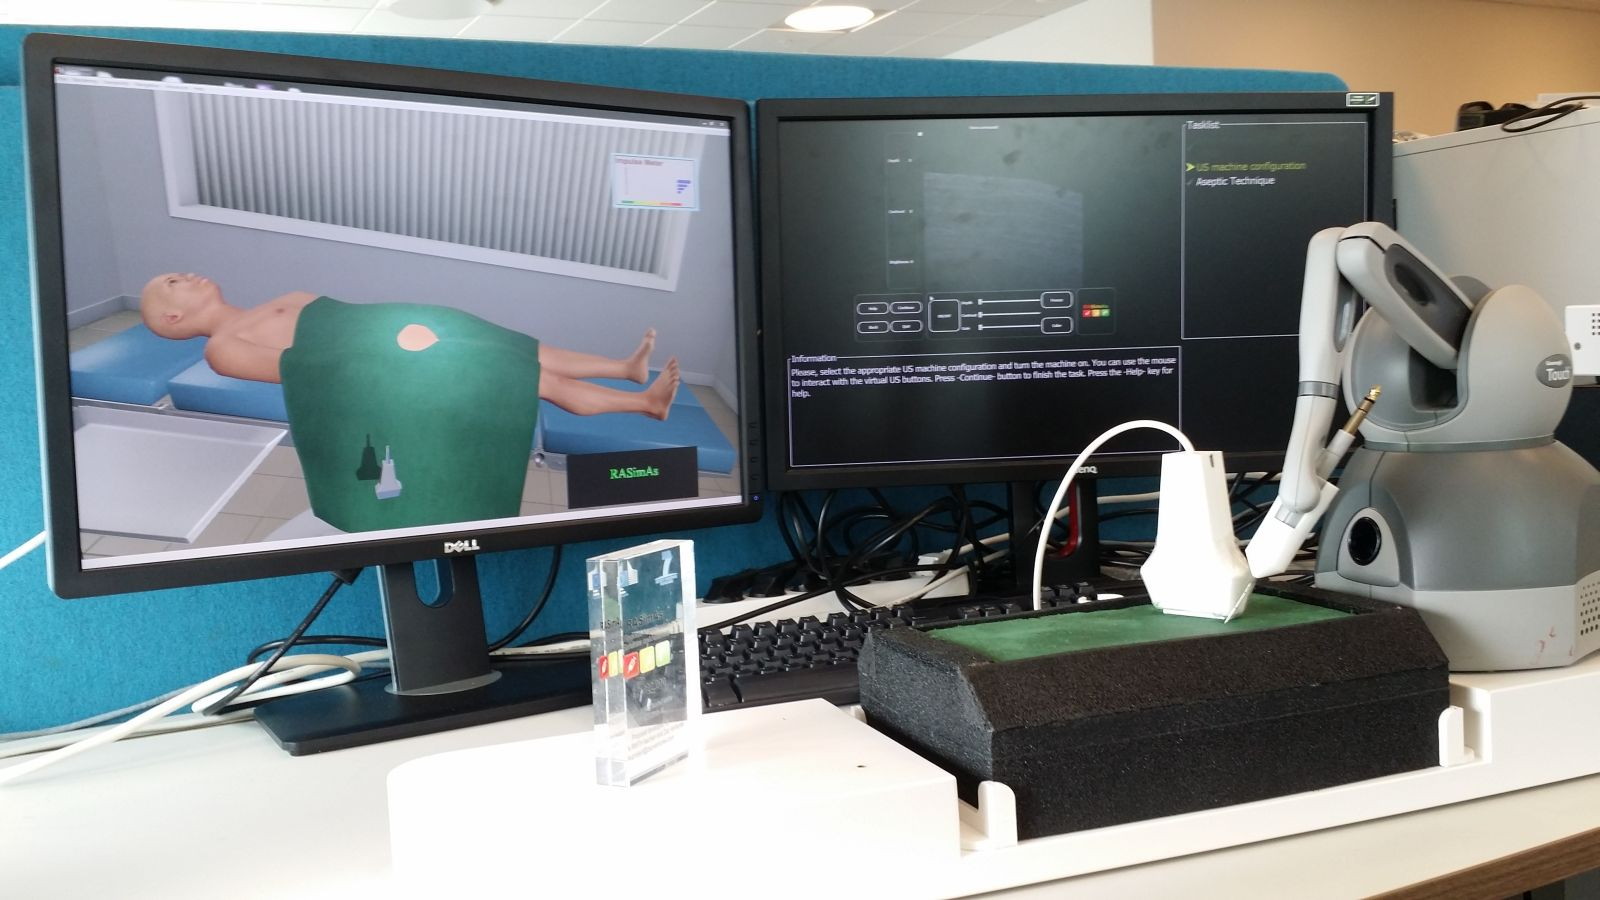
\includegraphics[width=0.9\textwidth]{IMG/sim3.jpg}
    \caption{\ac{RASim} \label{subfig:rasim}}
  \end{subfigure}%
  \begin{subfigure}[b]{0.5\linewidth}
    \centering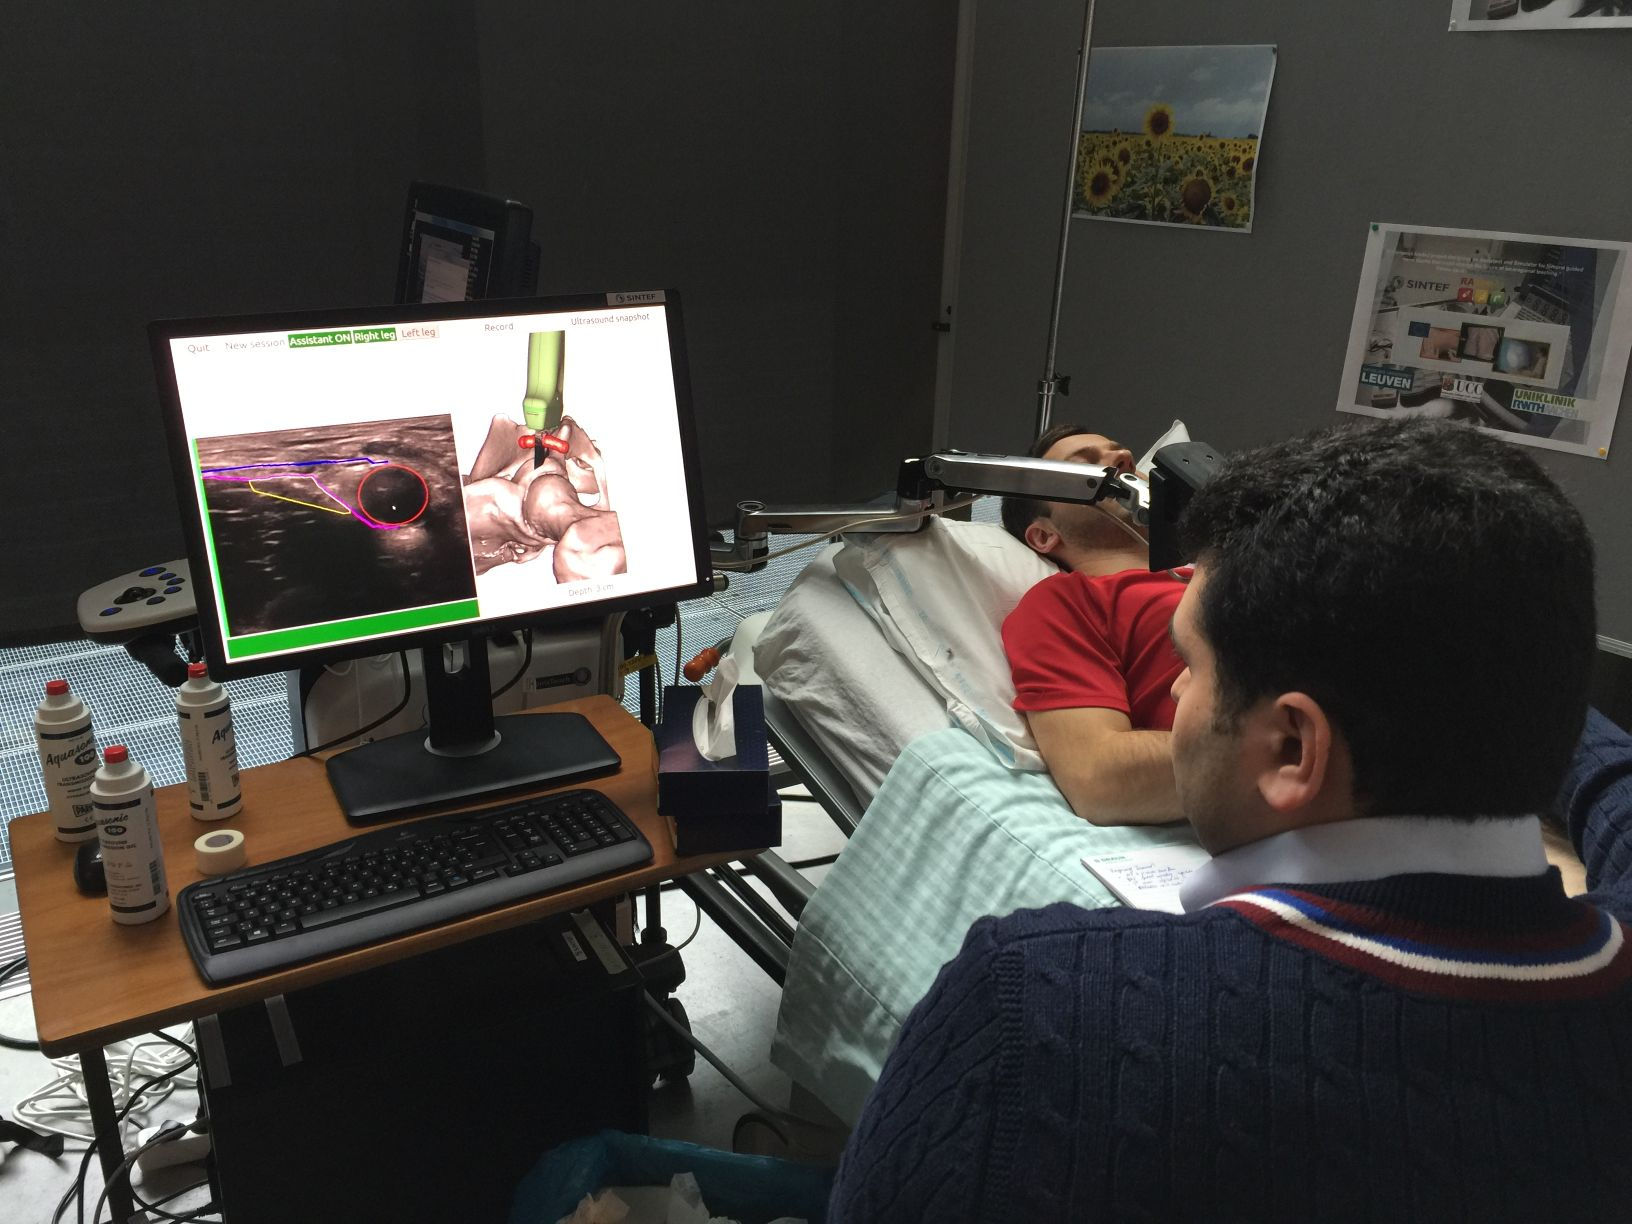
\includegraphics[width=0.9\textwidth]{IMG/raas.JPG}
    \caption{\ac{RAAs} \label{subfig:raas}}
  \end{subfigure}
  \caption{Imágenes que muestran los dos prototipos desarrollados en el contexto de \ac{RASimAs}}
\end{figure}

%https://www.openanesthesia.org/regional-anesthesia-curriculum/
%http://rasimas.imib.rwth-aachen.de/member_area/documents_ma/Extra_Material/ISRA_Anaesthesia_Foundation_Course_Book_v1_to_print_for_ISRA_course_Oct_2_2014.pdf
%\todo{ Pon alguna cita, aquí y en el estado del arte. Por ejemplo, el CV de RA de Cork. Esto luego lo usaras en el courseware}

La \ac{RA} es un procedimiento mínimamente invasivo en el cual el médico administra un anestésico local en las proximidades del nervio que se desea bloquear \cite{CVraisra}. Esta técnica, frente a la anestesia general y si se practica adecuadamente, reduce: los efectos adversos sobre el paciente, su tiempo de recuperación y el coste de la intervención \cite{PMID:26695878}. La dificultad principal del procedimiento radica en liberar el bolo anestésico alrededor del nervio, sin tocarlo, evitando liberar la dosis en el torrente sanguíneo y confirmar que éste se ha extendido correctamente a su alrededor. Actualmente, existen dos técnicas para guiar la aguja hacia su objetivo: la estimulación eléctrica del nervio y el uso de imagen por \ac{US}. Aunque ambas técnicas pueden combinarse, la tendencia actual es abandonar la electroestimulación en favor del guiado por \ac{US}.

% \del{La \ac{RA} es un procedimiento médico dónde el \del{anestesiólogo}\new{anestesista!!!!!} administra anestésicos locales al paciente, a través de una aguja guiada por \ac{US} \todo{ojo hay otras formas de guiado. Tienes que ser muy preciso} en áreas cercanas a nervios específicos, produciendo una disminución de su actividad y ausencia del dolor. Esto posibilita la realización de cirugías sin necesidad de dormir al paciente completamente. De esta manera, se puede reducir el dolor postoperatorio, mejora la recuperación postoperatoria y se reduce el tiempo de hospitalización. De hecho, la anestesia regional se está imponiendo frente a la anestesia general debido a su menor coste e impacto en el paciente. \todo{cita}}
Sin embargo, esta técnica no es sencilla para los anestesistas que no están familiarizados con la imagen por \ac{US}. Requiere tener una buena base teórica y práctica que permita proceder de manera segura. A día de hoy, está técnica se aprende principalmente practicándola sobre el paciente (\emph{by doing}), aunque existen otras técnicas como el uso de cadáveres\cite{Tsui2007} o \emph{fantomas}\footnote{castellanización del término inglés Phantom}\cite{phantomra}. Estas técnicas tienen claras limitaciones como: un alto coste, 
la imposibilidad de repetir escenarios, el aprendizaje auto-guiado, 
la imposibilidad de enfrentar la usuario a a una amplia variabilidad anatómica, ...
%\borrar{enfrentar al usuario a una amplia variabilidad anatómica, etc.}

En primer lugar, \ac{RAAs} es un sistema de guiado que superpone información adicional sobre la imagen de \ac{US}, ayudando al usuario a identificar distintas regiones de interés. El sistema dispone de un \ac{tracker} y de un análisis de imagen que ayudan al médico a reconocer la aguja, la trayectoria de esta y las estructuras anatómicas relevantes mientras se esta realizando la operación. 
% \del{Respecto a el sistema de guiado \ac{RAAs} consiste en asistir al anestesiólogo durante el procedimiento de \ac{RA}. Este sistema consta de unos dispositivos de seguimiento incorporados en la aguja y en la sonda del \ac{US}, de tal manera que con la información de seguimiento y la imagen de \ac{US}, el asistente proporcionará retroalimentación de inmediato que ayudará al médico a interpretar la imagen de \ac{US} de la anatomía del paciente.}


%\todo{Rehaz este parrafo. 1. No entiendo porque solo destacas 2 modulos del sistema el haptico y el fantoma. No has hablado del curseware, de las métricas del modo guiado. Del modulo físico, del modulo de ultrasonidos. Estructuralo todo en partes Hw y Sw y detallalas todas. } 
%
\ac{RASim} es un simulador médico que recrea un entorno de \ac{RA} donde el usuario puede entrenar el procedimiento. El usuario se sitúa en frente de la mesa de trabajo donde podrá encontrar: un maniquí y los dispositivos de \ac{E/S}.
El usuario interacciona con el sistema a través de una sonda de \ac{US}, con un \ac{tracker} magnético incorporado, y una aguja, acoplada a un dispositivo háptico. Estos dispositivos permiten al sistema seguir los movimientos del operador y proporcionar una respuesta háptica (en el caso de la aguja).
El usuario puede seguir el avance del procedimiento gracias a dos pantallas. En una, se muestra una vista virtual de la sala de operaciones  y, en la otra, se muestra el interfaz de la \ac{Courseware}\footnote{Es un software diseñado para fines educativos que sirve como ayuda o refuerzo del contenido} con la imagen simulada de \ac{US}.
%
\todo{Tienes que rehacer todo de aquí al final del párrafo. 1 Enu,era todos los modulos SW. Luego si quieres explica todos ellos. Pero no te metas en mucho detalle. Los detalles van al capitulo de RASim.  }
\new{Así mismo, el simulador se compone de varios módulos software:}
\begin{itemize}
    \item Módulo de respuesta háptica para la aguja.
    \item Simulación física entre los tejidos y los instrumentos médicos.
    \item Módulo de simulación de imágenes de \ac{US}.
    \item Renderizado de la escena virtual.
    \item Plataforma de autoevaluación y aprendizaje (\acs{Courseware}).
\end{itemize}

Es importante destacar, que el módulo de \ac{Courseware} es el que convierte al simulador en una plataforma de entrenamiento. Este software dirige al usuario a través del procedimiento mientras \new{coordina todos los módulos del simulador en función de las necesidades del entrenamiento. } 
%
El simulador permite practicar el procedimiento completo en un entorno seguro, además de mejorar sus habilidades cognitivas y no cognitivas gracias a la realimentación que proporciona el sistema.

Con el objetivo de enfrentar a los médicos a distintos escenarios que representen una variabilidad anatómica significativa, en el proyecto \ac{RASimAs}\new{ se ha propuesto desarrollar un entorno integrado de generación de pacientes virtuales (en inglés: \ac{ITGVPH}) con el que generar una base de datos que permite la creación de pacientes virtuales medios, utilizables en \ac{RASim}. }
%
\todo{Esta frase no tiene sentido 1. estructuras anatomicas, para generar modelos anatomicos 2. Que son las estructuras mecanicas?. Lo suyo es resumir el procedimiento de creación del paciente virtual o enumerar sus etapas.}
\new{Esta herramienta genera \ac{VPH} representativos a partir de un registro entre un modelo virtual comercial e imágenes de pacientes reales. También es capaz de generar el comportamiento mecánico  de los tejidos necesario para su simulación física, y, adicionalmente, cambiar la postura inicial del paciente virtual a la posición requerida por el procedimiento.}
%\new{Por otra parte, este mismo sistema puede ser usado como plataforma de entrenamiento autoguiado en la que el usuario puede practicar el procedimiento gracias a la retroalimentación que el sistema proporciona.}

%Se ha diseñado una mesa de trabajo donde el usuario interacciona con el sistema. En ella, se encuentran dos pantallas que sirve para proporcionar información visual al usuario. En una de ellas se puede visualizar una vista de la sala de operaciones virtual y en otra, se muestra la vista del software de entrenamiento junto con la imagen simulada de \ac{US}. En la mesa de trabajo, el usuario maneja una sonda de \ac{US}, con un \ac{tracker} magnético incorporado, y una aguja, acoplada a un dispositivo háptico, que permite al sistema el seguimiento de los movimientos del usuario. El simulador es capaz de simular la interacción y deformación de los instrumentos y tejidos, y generar una imagen de \ac{US}. El \ac{Courseware} es el encargado de dirigir al usuario a través del procedimiento y gestionar todos los modulos del simulador. 

%\todo{tienes que restructurar toda la información de RASim. 1. Objetivos (no uses la palabra objetivos todo el rato):variabilidad anatómica gran base de datos de pacientes, aprendizaje autónomo, autoevalucaion (no digas evaluación es demasiado ambicioso). 2. Modulos Hw y Sw. Importante: no me lo vuelvas a pasar hasta que lo hayas leído 3 veces. No puedo dedicar tanto tiempo a cada capítulo. Ojo Con las afirmaciones como modulo realista (si no esta evaluado, no lo sabes. Por otro lado, el módulo haptico es una mierda). }
%El objetivo de este simulador es que el usuario pueda aprender el procedimiento completo en un entorno seguro y además pueda practicar sus habilidades cognitivas y no cognitivas en el sistema. 
%\todo{demasiado ambicioso}
%de las capacidades de los profesionales, gracias a los dispositivos hápticos y a la simulación física la cual es capaz de recoger parámetros de rendimiento más allá de valoraciones subjetivas que podría tener un supervisor.\todo{No dices nada de autoguiado, ni de autoevaluación.}






%\subsection{Contribuciones al proyecto RASimAs}
%\label{intro:context}

\begin{figure}
    \centering
    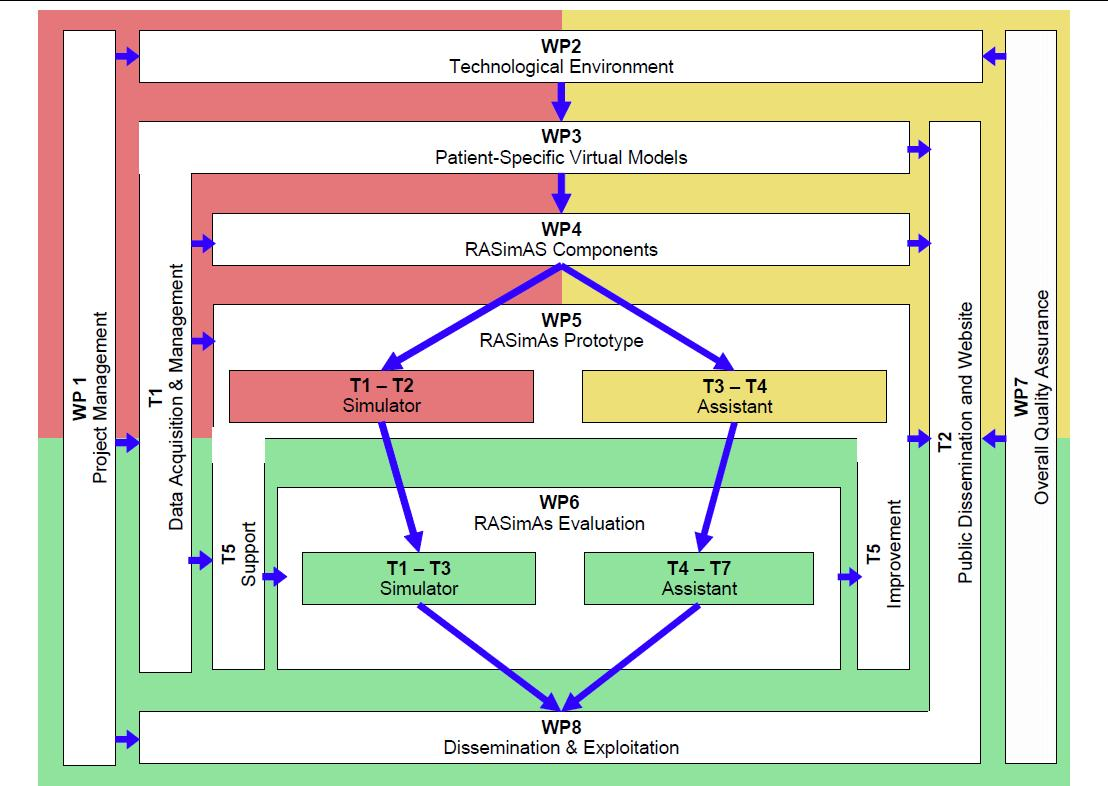
\includegraphics[width=0.95\textwidth]{IMG/wp_overview.jpg}
    \caption{División y organización de los \acl{WP} de \ac{RASimAs}}
    \label{fig:wp_rasimas}
\end{figure}

El proyecto \ac{RASimAs} se organiza en los ocho \ac{WP} que se pueden observar en la figura \ref{fig:wp_rasimas}. Los \ac{WP} 1, 7 y 8 se encargarán de tareas de gestión: coordinación, control de calidad, diseminación de resultados y explotación de los prototipos. El \ac{WP} 2 desarrollará la plataforma donde se integrarán todos los módulos de software y datos generados de los siguientes paquetes. En los \ac{WP} 3 y 4 se desarrollarán los componentes necesarios de los dos prototipos que se implementan en el \ac{WP} 5. Por último, el \ac{WP} 6 se encarga de la evaluación clínica tanto del prototipo de \ac{RASim} como del \ac{RAAs}. 

\new{En el capítulo \ref{cap:rasim} , se introducirán los \ac{WP} 3, 4 y 5 y las tareas en las que ha contribuido de manera activa la \ac{URJC} y donde se encuadra la mayor parte de la investigación realizada en esta tesis.}


\subsubsection{Colaboración con la \acl{Bangor}}
%\todo{Aaron, se que soy un pesado, pero cuando te digo que pienses cada frase me refiero a esto. El motivo por el que las colaboraciones entre miembros del proyecto van más allá de las tareas del mismo, NO es que trabajen distintas instituciones, SINO que estos proyectos permiten conocer de forma más próxima el trabajo que se está realizando en otros laboratorios }
%\todo{Para nada considero que seas pesado, al revés, el conformista soy yo...}
%
Uno de las ventajas que tienen los proyectos internacionales de esta índole es que mejora la visibilidad del trabajo realizado por los miembros del consorcio, fomentando colaboraciones entre socios más allá del ámbito del proyecto.
%
En el caso de este trabajo de tesis, \ac{RASimAs} proporcionó la oportunidad de conocer en profundidad el trabajo del  Dr. Franck P. Vidal, miembro del  \emph{School of Computer Science} de \acl{Bangor}, en el campo la simulación en tiempo real de la generación de imágenes médicas de rayos X \cite{villard2014interventional}. El Dr. Frank P. Vidal es el responsable de la librería \emph{gVirtualXRay}\cite{sujar:hal}.
%
A partir de esta tecnología y la herramienta de posicionamiento de pacientes, creada en el contexto del proyecto \ac{RASimAs}, se propuso desarrollar un simulador de radiología diagnóstica en el que seguir evaluando la viabilidad de los algoritmos propuestos en este trabajo.
%que utilizará los dos módulos para permitir a un usuario practicar el posicionamiento de un paciente por parte de un radiólogo.
La radiología es una especialidad de diagnóstico por imagen que utiliza la tecnología de los rayos X. Debido a la peligrosidad de una exposición prolongada a estos rayos, un simulador que permita al radiólogo entrenar de manera segura y que pudiera ser utilizado sin restricciones de tiempo, sería de gran utilidad en el campo.
Como resultado de esta colaboración, se han podido realizar dos estancias del autor de esta tesis en la \acl{Bangor}. 

%1. El proyecto Rasimas nos da la oportunidad de trabajar con miembros de la universidad de Bangor y conocer su trabajo.2. Frank School of Health Sciences y el otro School of Computer Science and Electronic Engineering3. Trabajan en radiologia (prescisa un poco dar mas detalles. Habla de sus publicaciones)4. Se plantea adpartar y extender las técnicas desarrolladas en el contexto de RaSimasç5. La colaboración se articula en dos estancias.}







\section{Motivación}
\label{intro:motivacion}
%\del{\todo{o pones citas o no haces estas aseveraciones} El uso de simuladores de realidad virtual en medicina es muy beneficioso al poder crear entornos seguros y reproducibles para los usuarios\todo{ una cita}. El auge que han tenido estos simuladores es gracias a su idoneidad para el entrenamiento y la enseñanza de los procedimientos médicos, consiguiendo una gran aceptación en todos los campos de la medicina\todo{cita}.  Aun así, la diversidad de procedimientos y la complejidad del cuerpo humano y llevar a cabo cada tipo de simulación diferente son las principales dificultades que se presentan en un futuro a corto plazo.  Los principales problemas que se han encontrado en los diferentes simuladores médicos son los siguientes:}

%\todo{ 1. tienes que hablar de la importancia de tener una libreria de pacientes 2. de la necesidad adapatarlos a la pose de operación y 3 de las aplicacioens que necesitan modificar la pose en tiempo real.  Habla de los problemas de las ténicas de posing existentes. tienes que hablar de los problemas de posing a la hora crear librerías validas para un determinado procedimiento con una poses estática o la importancia de poder cambiar la pose en el procedimiento como con los x-ray. Indicar los problemas a la hora de modificar geometrias incompletas sin descripcion de comportamiento....}
%\todo{He visto que mucho de lo que te he dicho está en los párrafos siguientes. Reestructúralo y lo vuelvo a corregir. Recuerda. Todo lo que quieres que me vuelva a leer ponlo con new.}


En el contexto de la simulación para entrenamiento médico, es importante que un profesional sanitario en formación se enfrente a la mayor cantidad de casos y  variaciones anatómicas posibles. En general, los simuladores médicos utilizan modelos anatómicos propios y específicos que no representan toda la variabilidad posible para entrenar de forma adecuada un determinado procedimiento. 
%\new{y es por ello que su utilización quedaría sesgada y resultaría complicado generalizar este aprendizaje al ámbito médico real }.
Por ello, nuevas plataformas de entrenamiento médico están incorporando datos de pacientes reales en sus simuladores \cite{Willaert2012,Votta2013}. Este enfoque no está exento de problemas:
\begin{enumerate}
   %\item Los datos anatómicos de los pacientes virtuales son estáticos y representan poca variabilidad.
    %\item En cada simulador se suele crear modelos anatómicos específicos y no son transferibles entre ellos.
    \item \new{Ningún método de adquisición de imagen médica es capaz de registrar todos los tejidos de un paciente.\todo{yo pondría ejemplos} Si bien es cierto que se podrían combinar datos procedentes de distintas técnicas es poco habitual dado que se presentan problemas de: coste, registro de imágenes, técnicas contraindicadas para algunos pacientes (por ejemplo el \ac{TC} abdominal en embarazadas)...}
    \item A partir las distintas técnicas de imagen médica es difícil obtener las propiedades mecánicas de todos o alguno de los tejidos registrados.
    \item Es habitual que las imágenes médicas se capturen con en paciente en una posición distinta a la requerida en la intervención.
    \item No siempre están disponibles información específica del paciente o solo se trata de una zona concreta del paciente. \todo{No entiendo este punto}
\end{enumerate}
%
Por todo lo anterior, el objetivo de \ac{RASimAs},  no es crear una base de datos de pacientes reales, sino de pacientes virtuales en la que estén representadas el mayor numero de representaciones anatómicas posibles. Estos pacientes virtuales se construirán promediando datos provenientes de pacientes reales. Puesto que no se trata de ensayar el procedimiento en un paciente real, el método, que adapte la pose de los pacientes virtuales a la requerida en el procedimiento, no tiene porque ser precisó desde el punto de vista fisco. Basta con que el resultado sea plausible, permitiendo al médico en formación entrenar de forma efectiva.
%\del{Por tanto, se hace necesario disponer de algún método que pueda capturar variaciones anatómicas, de tal manera que pueda incorporarlas al simulador que se estuviera utilizando. En este caso, en lugar de tener un modelo anatómico con una configuración concreta, % En la motivación, cuando hables de la base de datos, di que en muchas aplicaciones lo importante es la variabilidad anatómica, no trabajar con pacientes reales. }
%basta con poder transformar cualquier modelo de paciente virtual existente a una pose plausible, pudiéndose utilizar en cualquier simulador que así lo requiera. De esta forma, se intenta abarcar la mayor cantidad posible de situaciones que puedan ayudar a los aprendices a mejorar su entrenamiento y por tanto su profesionalidad .}
 
Cabe destacar que, dentro de la generación de imágenes por computador, existen diferentes técnicas para poder animar personajes virtuales. 
\del{Es habitual que estos métodos sean utilizados para animar estructuras anatómicas con diversas finalidades como pueden ser: cinematográfica, lúdica o sanitarias.}\todo{esta frase no es verdad.} 
Estas técnicas suelen estar divididas comúnmente entre métodos geométricos y métodos basados en física. Ambos enfoques presentan ventajas \new{e inconvenientes} \del{sobre los otros} y su uso \new {dependerá de} \del{se extiende en base a} sus características. 

Considerando los problemas citados anteriormente y \new{las restricciones impuestas por el proyecto \ac{RASimAs} (ver apartado \ref{XXXXXXXX}), esta tesis pretende comprobar si es posible diseñar un método geométrico que permita entrenar en el entrono medico de forma efectiva.}\del{dentro del contexto del proyecto europeo \ac{RASimAs}, la motivación de esta tesis es comprobar si es posible diseñar un método geométrico que pueda solventar determinados problemas.} A continuación, se muestran las diferencias \new{entre ambas aproximaciones}\del{que tienen las técnicas geométricas frente a los métodos basados en físicas:}

\begin{itemize}
\item Los métodos basados en \new{modelos físicos}\del{físicas} se centran en conseguir deformaciones \new{plausibles}\del{realistas REALISTAS NO QUIERE DECIR NADA}, frente a los geométricos que proporcionan soluciones plausibles. \new{Es decir, deformaciones que el usuario pueda interpretar como reales.} 
%\todo{esto es una ventaja? quizás habría que poner arriba en vez de ventajas, diferencias}
%OK


\item Los algoritmos geométricos son más robustos\new{. En la mayoría de los casos son soluciones \emph{ad hoc} que no sufren de los problemas de estabilidad de los métodos numéricos que se utilizan para resolver las ecuaciones diferenciales que modelan el comportamiento de los distintos objetos físicos. }\del{ante la falta de una descripción completa de un modelo anatómico. Debido a las dificultades que tienen la adquisición de imágenes médicas, no es habitual que todas las estructuras anatómicas estén presentes o se puedan capturar el comportamiento de todas ellas.}

\iten \new{Por otro lado, los métodos basados física requieren caracterizar mecánicamente los modelos que se van a simular. Está información no siempre puede obtenerse de forma precisa a partir de las imágenes médicas.}

\item \new{Debido a la complejidad de los comportamientos que deben simularse, la mayoría de los algoritmos biomecánicos actuales se centran en el comportamiento de estructuras concretas, como por ejemplo los sistemas de animación musculo-esqueleto que obvian las interacciones con otras estructuras. }

\item Es habitual que los métodos geométricos tengan tasas de refresco altas, en comparación a los algoritmos basados en física\del{s}. Estas técnicas habitualmente son demasiado costosas para conseguir interactividad\del{, sea necesario la intervención de un usuario dado su complejidad o se centren en una zona limitada de la anatomía??????????????????????}.\new{El problema se agrava  cuanto más complejos sean los comportamientos que se quieran simular. Destacar que la simulación biomédica tiene un alto grado de complejidad debido a la variedad de estructuras y comportamientos mecánicos a simular.}

\item \del{Debido a su popularidad, actualmente los métodos geométricos están diseñados para aprovechar totalmente la arquitectura de las tarjetas gráficas.}
    
\item \del{Los modelos basados en físicas están muy extendidos, aunque en su gran mayoría se centran solo en el sistema \new{músculo-esquelético} \del{musculoesqueletal}.} \todo{El sistema locomotor, llamado también sistema músculo-esquelético.}
\end{itemize}

Disponer de un método geométrico que permita adaptar la postura a modelos anatómicos humanos ayudará a:

\begin{itemize}
    \item Poder modificar cualquier modelo virtual con estructuras anatómicas internas a la posición requerida por un procedimiento médico.
    \item \new{Poder adaptar cualquier pacientes virtual aunque este presenten tejidos incompletos o cuyas propiedades mecánicas no hayan sido registradas.}
    \item \del{El método permite una interacción inmediata y servirá para utilizarse en simuladores de entrenamiento médico????}
    \item \todo{Su flexibilidad y su rapidez le hacen posible incorporarlo en cualquier simulador o herramienta de \ac{RV}. REDACTA BIEN}
\end{itemize}


\section{Hipótesis de partida} 
\label{intro:hipotesis}
%\todo{la hipótesis de partida es buena}
Con las motivaciones anteriormente descritas, se procede a formular la siguiente hipótesis de partida:

%\emph{es posible crear un método geométrico para animar modelos anatómicos humanos en tiempo real del que no se posean completamente todos sus tejidos o propiedades mecánicas que pueda ser utilizado en simuladores médicos para entrenar nuevos médicos. }

%\emph{ En el contexto del entrenamiento en simuladores médicos, se pueden diseñar algoritmos geométricos capaces de adaptar la antinomia del paciente virtual a la pose requerida en el procedimiento simulado de forma que la transferencia de competencias sea efectivo.}

\begin{center}
    \begin{minipage}{0.9\linewidth}
        %\vspace{5pt}%margen superior de minipage
        {\small
\emph{es posible diseñar un algoritmo geométrico capaz de adaptar modelos anatómicos de un paciente virtual desde una posición inicial a la pose requerida por un procedimiento médico y que sirvan para que la transferencia de competencias sea efectiva en el contexto de formación utilizando simuladores de realidad virtual. }
        }
        %\vspace{5pt}%margen inferior de la minipage
    \end{minipage}
    
    
\end{center}




% Hipótesis:
% -        Método geométrico puede ser utilizado en el contexto de los médicos:
% o   Datos incompletos (geométricos y mecánicos)
% o   Velocidad para el tiempo real. 
%o   Otras ideas

\section{Objetivos}
\label{intro:objetivos}
%\todo{Cuida más los objetivos. Mas o menos se entienden pero tienen que sonar claros y rigurosos.}
%Con la  cuando la posición del paciente en el momento que se adquiere una imagen médica (por ejemplo \ac{IRM} o \ac{TC}) es normalmente diferente a la posición requerida por el procedimiento médico que se este simulando. A la vez, estas imágenes suelen ser locales y no son capaces de recuperar cada uno de los tejidos del paciente o su comportamiento mecánico.

Con la hipótesis de partida enunciada, a continuación, se presentan los objetivos principales que se pretenden alcanzar a lo largo de la presente tesis:

\todo{Asegurar que todo esta escrito en futuro}
\begin{itemize}
\item Diseño de un algoritmo para el posicionamiento de modelos anatómicos, desde la posición en la que fueron modelados hasta cualquier posición requerida.
\\
%\todo{no puede ir en pasado son objetivos!!!!. Escríbelos como tales}

Se propondrá una técnica que permita transformar los modelos anatómicos de pacientes virtuales, los cuales originalmente se encuentran en una postura diferente a la posición necesaria para el entrenamiento de un determinado procedimiento médico. %\todo{desde la coma suana raro}. 
La técnica propuesta será capaz de modificar un modelo anatómico con estructuras internas de manera interactiva, siendo esto posible, aunque el modelo no fuera completo o no estuvieran disponibles las propiedades mecánicas de los tejidos. En resumen, la técnica que se proponga deberá verificar los siguientes requisitos:
%\todo{sin necesidad de disponer de una descripción mecánica de las porpiedades de los tejidos y incluso sin disponer de un modelo completo, es decir, no es necesario que estén modeladas todas las estructuras anatómicas. (Pon esto bonito)}

\begin{itemize}
%\todo{Yo aquí subdividirá el objetivo 1 en los requisitos de la técnica}
    \item Debe funcionar en tasas interactivas.
    \item Debe poder trabajar con modelos incompletos.
    \item No necesita las descripciones mecánicas de los tejidos.
    
\end{itemize}

%\todo{Tenemos que hablar.  2. La idea es probar el algortimo en dos casos de uso reales. Uno que demuestre que funciona con información incompleta y otro que demuestre que funciona en aplicaciones interactivas. Ojo con decir que probamos que la transferencia de conocimientos es adecuada, no lo hacemos!!!!. Tienes que insinuarlo sin dejarlo explicito.

\item 	Validación del algoritmo. \\
%\todo{Yo diría en los objetivos que la técnica servirá para entrenar si se al incorporarla en simuladores estos pueden usarse para entrenar.}
%\todo{Los objetivos son muy importantes. Redacta esto mejor. }
Con el fin de demostrar que el algoritmo propuesto pueda ser utilizado en el entrenamiento médico, este será incorporado en dos tipos de aplicaciones de \ac{RV}. En el primer caso, se intentará demostrar que el algoritmo puede adaptar la postura de un modelo anatómico en un escenario donde no se dispone de modelos completos desde un punto de vista anatómico y en los que tampoco se disponga de los parámetros que caracterizan el comportamiento mecánico de las estructuras presentes. En el segundo caso de uso, el algoritmo mostrará su utilidad en un entorno donde el usuario deberá modificar interactivamente la posición del paciente como parte del procedimiento. 

%Objetivos secunadrios:

%- Objetivos del algoritmo

%- Objetivos de los dos casos de uso.

%--- Recureda. En el simuladador de anestesia regional no se cambia la pose en tiempo real (validamos descripciones incompletas)

%--- El de radiología la selección de la pose es parte del comportamiento, aunque por otro lado hay menos estructuras anatomicas relevantes.

\begin{itemize}
    \item 	Caso de uso: Simulador de anestesia regional y herramienta \ac{ITGVPH}
    %\todo{No me gusta que lo vendas como offline. Hemos vendio que un experto valida la pose por lo que la herramienta itne que ser interactiva.}:
    
    Un objetivo del proyecto \ac{RASimAs} es la creación de la herramienta \ac{ITGVPH} para generar una base de datos con pacientes virtuales que representen distintas variaciones anatómica promedio y que posteriormente será utilizada en \ac{RASim}.
    El algoritmo propuesto se integrará y comunicará con otros módulos que componen la herramienta, permitiendo animar y adaptar los \ac{VPH} generados. El método estará en comunicación con otros módulos desarrollados dentro del proyecto \ac{RASimAs}. Además, se desarrollarán los módulos del simulador con la finalidad de comprobar si la generación de estos \ac{VPH} es útil para entrenar el procedimiento de \ac{RA}.
    
   % \del{Además, se desarrollará un \emph{software} (\acs{Courseware}) para el simulador \ac{RASim} que se encargará de la comunicación con los demás módulos, y gestionará la interacción del usuario en una plataforma de entrenamiento auto guiada.}\todo{El courseware no es un objetivo. Lo que haces es desarrollar modulos del simulador de cara que este pueda utilizarse para entrenar a pacientes. No des muchos más detalles.} 

%\todo{Idea, no se necesitan pacientes reales sino pacientes medios. No se necesita una deformación presica, sino plausible}

%\todo{No entiendo este segundo parrafo. Puedes hablar del curseware. No se porque hablas de los hapticos y del Hw eso va antes?????}
    

    \item Caso de uso: Simulador de radiología diagnóstica

%\todo{Lo que tienes que vender aquí es que el posing del paciente es parte integral del procedimeinto y que se requiere un algorimo robusto que funcione en con tasas de refresco interactivas.}
%En este caso de uso, el algoritmo propuesto permite al usuario modificar la postura del paciente con el objetivo de entrenar el procedimiento de radiología diagnóstica.\todo{no has dicho nada} 
En radiología diagnóstica, el médico debe posicionar al paciente y configurar la máquina de rayo X de manera que la región anatómica objeto de estudio sea adecuadamente capturada. El algoritmo propuesto permite modificar la posición de un paciente virtual interactivamente, permitiendo probar distintas proyecciones y obtener imágenes de rayos X simultáneamente. El simulador permitirá entrenar las proyecciones radiográficas sin ningún riesgo para el paciente o el usuario. Este simulador, podrá ser usado tanto por profesores como por estudiantes de radiología como una herramienta adicional a las técnicas clásicas de aprendizaje.
\end{itemize}

\end{itemize}

% \begin{itemize}
%     \item 	Diseño del entrenamiento y evaluación del simulador.
% \end{itemize}

% La \ac{RV} proporciona una herramienta muy útil para poder guiar y ayudar en el proceso de aprendizaje al usuario. Mediante tareas guiadas, el usuario podrá aprender y perfeccionar el procedimiento quirúrgico, que ayudará a suavizar así la curva de aprendizaje y reducir posibles riesgos en el futuro. El simulador permitirá empezar por los caso más sencillos e ir facilitando el entrenamiento de casos más complejos. El objetivo es, que el usuario aprenda desde las competencias más básicas hasta simulaciones de situaciones reales, intentando minimizar el tiempo de aprendizaje. El usuario puede repetir el entrenamiento hasta que adquiera las habilidades requeridas. Debido a que cada vez más están presentes los simuladores en el currículum de los estudiantes de medicina, es necesario  crear unas métricas que sean útiles para evaluar a los estudiantes de manera cualitativa.




\section{Contribuciones}
\label{intro:contribuciones}

La principal contribución de esta tesis es la presentación de un algoritmo geométrico que permite modificar un modelo de paciente virtual de una postura original a la posición requerida por cualquier simulador. Este algoritmo ha sido diseñado, creando y adaptando técnicas establecidas en el cauce clásico de la animación esqueletal, pero permite animar tanto los modelos superficiales clásicos como los tejidos internos de un modelo de un paciente virtual.

El algoritmo propuesto es capaz de solucionar dos grandes problemas que se pueden encontrar un usuario al animar anatomía humana. Por una parte, esta técnica es capaz de manejar datos incompletos, tanto por la imposibilidad de capturar todos los tejidos dentro de la anatomía, %\todo{parece que hay gente que va por ahí sin pulmones} 
como por la falta de una descripción mecánica de los tejidos a animar. Esta característica ayuda a resolver casos donde los modelos procedentes de imágenes médicas %\ac{parciales}\todo{lo de locales no está suficientemente justificado}
que no contengan la descripción del paciente al completo. Por otra parte, esta técnica permite animaciones en tiempo real para que sea posible incorporarlo en cualquier simulador que lo necesite. El algoritmo es lo suficientemente rápido para mover la anatomía de un modelo de cuerpo entero permitiendo tasas interactivas al usuario.

Con el objetivo de demostrar la utilidad de la técnica propuesta, se ha procedido a incorporarla en dos simuladores médicos como ejemplos de casos de uso. 

\subsection{Contribuciones a RASimAS}

%\todo{Creo que le falta peso al curseware. YO DARIA PESO AL COURSEWARE AQUÍ NO EN LOS OBJETIVOS. LO MISMO EN EL SIMULADOR DE RAYOS X}
%es una de las motivaciones\todo{así suena raro} y parte financiadora de esta tesis,\todo{dos frases} el algoritmo propuesto es una parte importante dentro de la consecución del simulador que representa uno de los dos pilares del proyecto europeo.  

%\del{ \ac{TPTVPH} donde se encuentra varios procesos, desde el registro de los datos del paciente pasando por el proceso de completar los tejidos, la definición de las propiedades mecánicas para poder crear el \ac{VPH} y por último, el posicionamiento del modelo a la postura requerida para cada procedimiento.}\todo{falso el TPTVPH es nuestra herramienta}

La participación en el proyecto \ac{RASimAs} es el punto de partida del desarrollo de esta tesis. Se ha contribuido con la creación de un algoritmo que permite la adaptación de un \ac{VPH}, de una postura inicial a una final, de manera automática o supervisada por un experto.
El algoritmo propuesto ha sido integrado dentro del entorno \ac{ITGVPH}.
Esta herramienta proporciona los modelos que se van a utilizar en \ac{RASim}, permitiendo un entrenamiento del procedimiento de \ac{RA} con una base de datos de pacientes que disponga de una amplia variabilidad anatómica.

Por otra parte, también se ha contribuido en la creación del módulo \ac{Courseware}, que gestiona todos los componentes del simulador y se encarga de implementar todas las tareas de relacionadas con el entrenamiento. \ac{RASim} se compone de varios módulos software:
\begin{enumerate}
    \item El módulo de ultrasonidos \cite{Law2015} encargado de simular el proceso de generación de la imagen de \ac{US} que se usa para guiar la aguja a su objetivo.
    \item El módulo de la simulación física que se ha implementado extendiendo la funcionalidad de la librería \ac{SOFA}\cite{sofaweb} y que se encarga de modelar el comportamiento de la aguja con \cite{needleinsertion}, de sus interacciones con los tejidos del paciente y de dar una respuesta háptica.
    \item \emph{H3D} \cite{sensegraphics2012open} es el módulo encargado de la visualización de la escena virtual.
    \item El \ac{Courseware}, que proporciona una plataforma de aprendizaje donde el usuario podrá practicar y desarrollar sus habilidades no cognitivas.
\end{enumerate}
%\new{(i) ; (ii) ; y del (iii) .}    
Desde la \ac{URJC} se ha liderado el proceso de integración del \ac{Courseware} en el simulador, debido a que es necesario una continua comunicación entre los módulo anteriormente citados y la plataforma de entrenamiento. El \ac{Courseware} gestionará los distintos módulos citados con la finalidad de permitir un entrenamiento autónomo y proporcionar retroalimentación formativa y sumativa, gracias a las métricas recogidas a través de estos módulos.

En las últimas etapas del proyecto, el comité médico del proyecto no valoró positivamente la respuesta háptica, no siendo posible su evaluación clínica. Debido a problemas de precisión de los dispositivos hápticos (presentaban defectos de fábrica), los médicos consideraron que podría introducir sesgos en los aprendices. A partir de una propuesta de la \ac{URJC}, se procedió a sustituir los dispositivos hápticos por unos \acs{tracker}s magnéticos que permitió conseguir una evaluación favorable por parte de los evaluadores.


% \todo{Explicar que:
% 1. El grupo de la URJC a liderado el proceso de integración.
% 2. Qué la plataforma haptica no contó on el visto bueno de los medicos implicados en proyecto. (Explica los problemas)
% 3. Indica que como parte de está tesis sutituiste el modulo haptico por un sistema basado en tracker magenticos que si conto con la aprobación de los medicos. }


\subsection{Simulador de radiología diagnóstica}
%El algoritmo presentado en esta tesis permite ser incorporado en cualquier simulador que requiera transformar la postura de un modelo anatómico con estructuras internas interactivamente.
%\todo{es muy repetitivo}
Como resultado de la colaboración con el Dr. Franck P. Vidal, se ha desarrollado un simulador de radiología diagnóstica con la librería \emph{gVirtualXray}\cite{sujar:hal} y el algoritmo propuesto. Esta herramienta interactiva permite practicar las proyecciones radiológicas de manera segura y sin necesidad de pacientes reales.  El simulador podrá ser usado tanto por los profesores como por los estudiantes de radiología, complementado así el material utilizado en clase. Con el objetivo de practicar con una amplia variabilidad anatómica, el algoritmo propuesto ofrece la posibilidad de incorporar modelos de pacientes virtuales creados externamente. Para ello, cuenta con preproceso que permite preparar los pacientes virtuales para el algoritmo teniendo unos requisitos mínimos. Esta etapa se ejecuta de manera automática y solo se ejecuta una vez por modelo.

%\todo{Indica que gracias a la flexibilidad del algoritmo de posing se han integrado distintos modelos creados por terceros y que el simulador permite la incorporación de nuevos modelos con un numero de restricciones mínimas, aplicando un pre-proceso en su mayor parte automatico.}



%\todo{intenta acortar la frase.}
Al igual que \ac{RASim}, se ha desarrollado un \ac{Courseware} que permite al usuario practicar el procedimiento de forma guiada y autónoma a la vez que permite al profesor diseñar ejercicios de clase. Finalmente, se realizó un estudio para validar su utilidad. 18 participantes realizaron una encuesta donde se les enseñaba las funcionalidades del simulador y se les preguntaba acerca de su opinión. Los resultados obtenidos sugieren que el simulador es lo suficientemente realista para que sea útil como herramienta de enseñanza y entrenamiento del procedimiento.
%\todo{Yo también explicaría que el simulador esta pensado como herramienta de clase puesto que su uso como entranador 

\todo{Si conseguimos la validación la ponemos aquí}
%\todo{requeriria una validación que va más allá del ambito de esta tesis aunque la funcionalidad de entrenamiento ha sido implementada. Aaron: Al final no he validado nada entonces? Quizás sea mejor no ponerlo aquí}
%\todo{Explica un poco el curseware y/o los modos de funcionamiento...}


%cuales son mis contribuciones al simulador y que módulos han sido cogidos 


%\appendix
%\include{appendix}
\cleardoublepage
% Como incorporar como un capitulo mas en el indice de la bibliografia
\addcontentsline{toc}{chapter}{Bibliografía}
\bibliography{bibliography}
\bibliographystyle{alpha}
\end{document}
